\begin{frame}
\LARGE{\centering
\textbf{Helicity correlates with relaxation times} \\
}
\begin{center}
 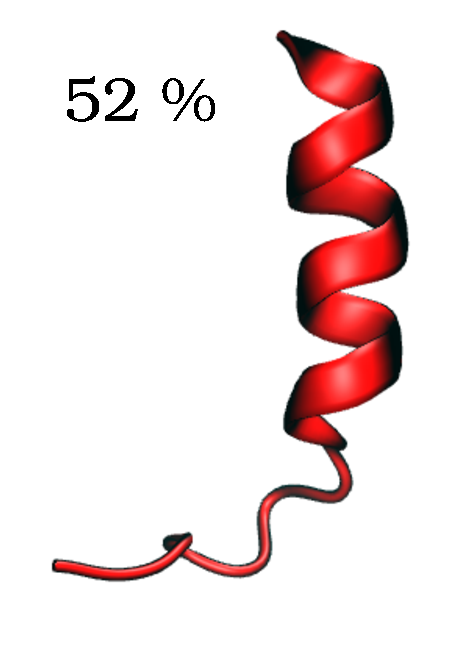
\includegraphics[height=4.5cm]{plots/helix1.pdf}
 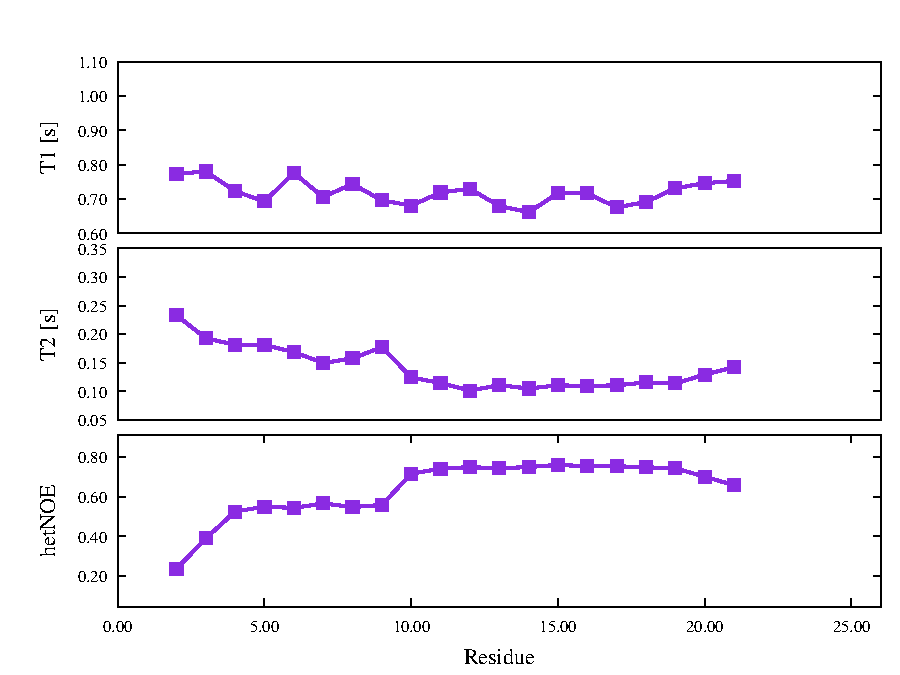
\includegraphics[height=5cm]{plots/simul_helix11.pdf}
 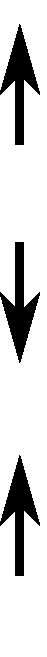
\includegraphics[height=4.5cm]{plots/arrows.pdf}
\end{center}
\end{frame}

\addtocounter{framenumber}{-1}
\begin{frame}
\LARGE{\centering
\textbf{Helicity correlates with relaxation times} \\}
\begin{center}
 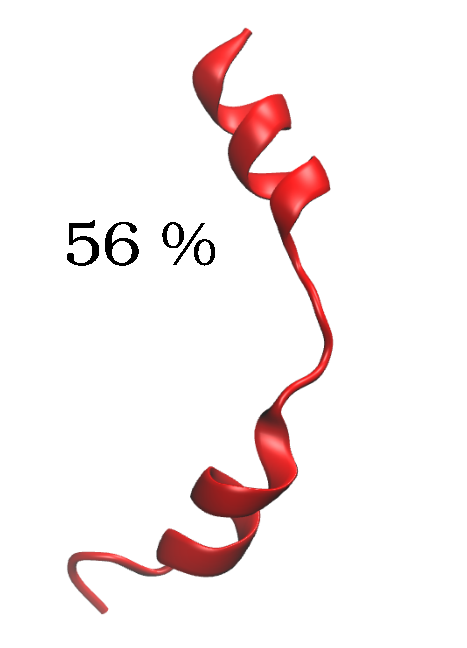
\includegraphics[height=4.5cm]{plots/helix2.pdf}
 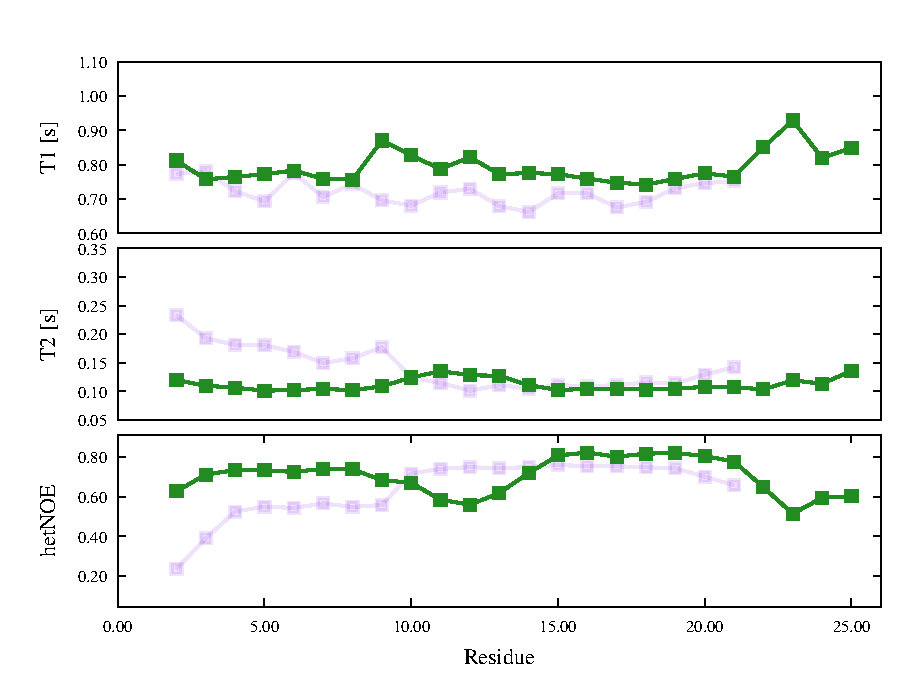
\includegraphics[height=5cm]{plots/simul_helix12.pdf}
 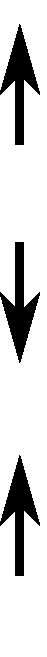
\includegraphics[height=4.5cm]{plots/arrows.pdf}
\end{center}
\end{frame}



\addtocounter{framenumber}{-1}
\begin{frame}
\LARGE{\centering
\textbf{Helicity correlates with relaxation times} \\}
\begin{center}
 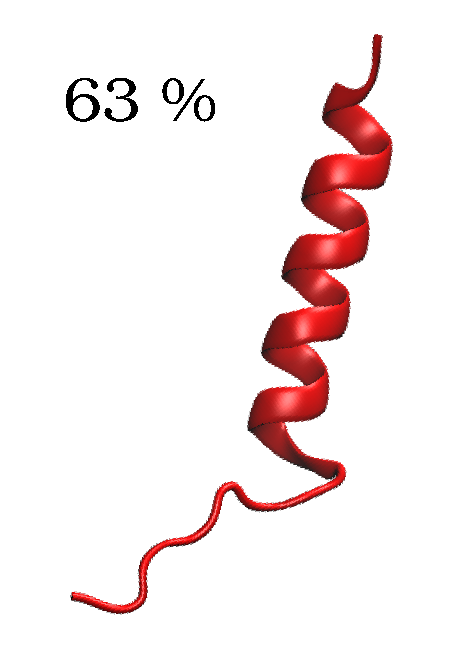
\includegraphics[height=4.5cm]{plots/helix3.pdf}
 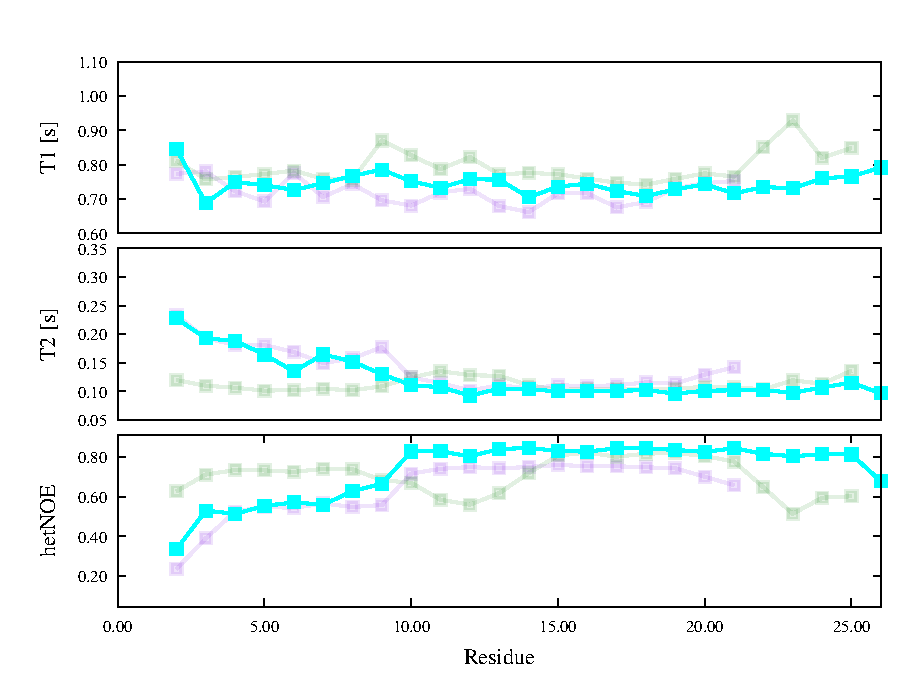
\includegraphics[height=5cm]{plots/simul_helix13.pdf}
 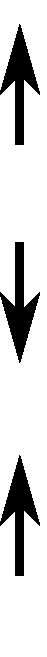
\includegraphics[height=4.5cm]{plots/arrows.pdf}
\end{center}
\end{frame}



\addtocounter{framenumber}{-1}
\begin{frame}
\LARGE{\centering
\textbf{Helicity correlates with relaxation times} \\}
\begin{center}
 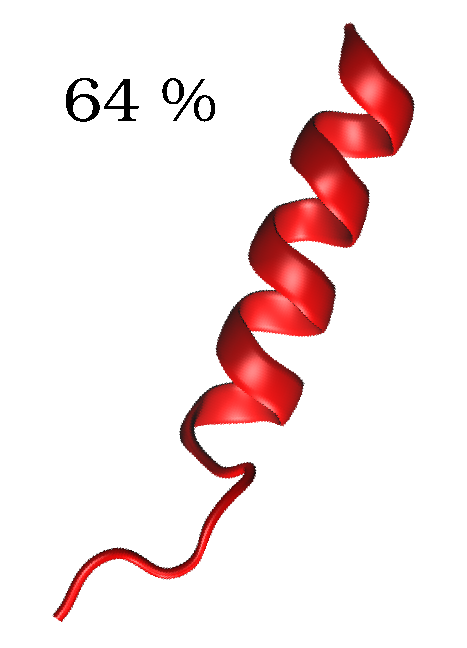
\includegraphics[height=4.5cm]{plots/helix4.pdf}
 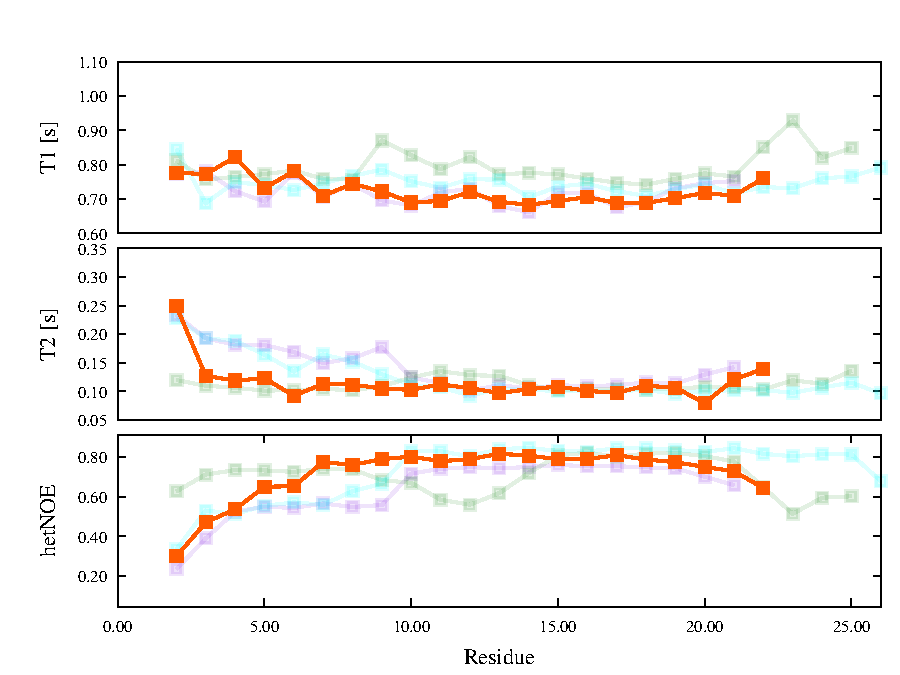
\includegraphics[height=5cm]{plots/simul_helix14.pdf}
 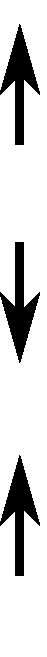
\includegraphics[height=4.5cm]{plots/arrows.pdf}
\end{center}
\end{frame}


\addtocounter{framenumber}{-1}
\begin{frame}
\LARGE{\centering
\textbf{Helicity correlates with relaxation times} \\}
\begin{center}
 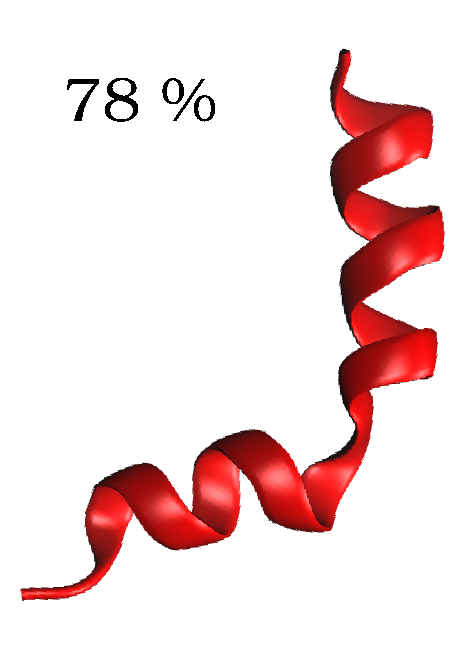
\includegraphics[height=4.5cm]{plots/helix5.pdf}
 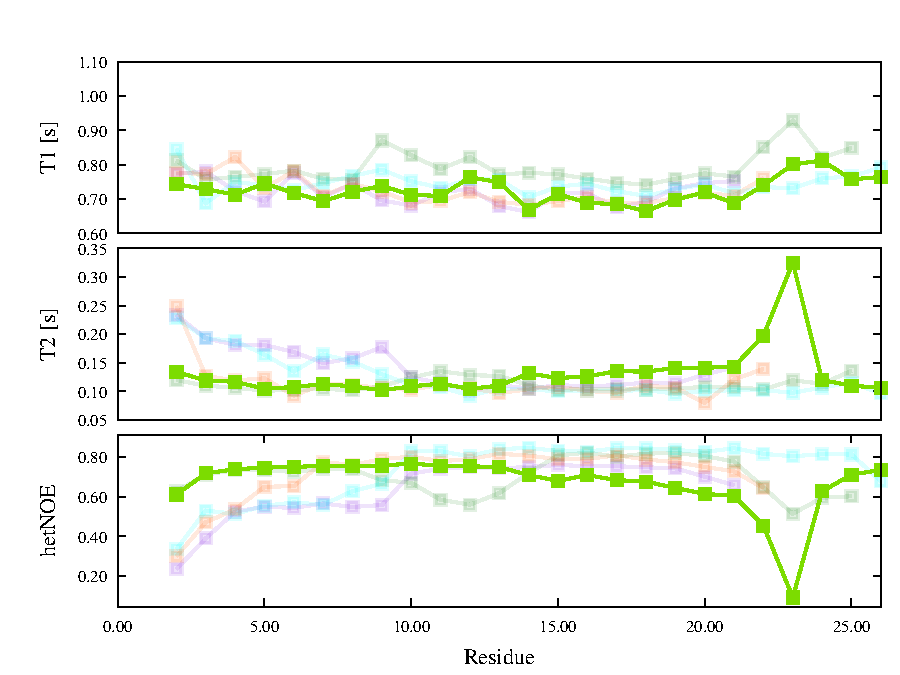
\includegraphics[height=5cm]{plots/simul_helix15.pdf}
 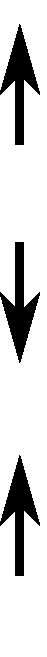
\includegraphics[height=4.5cm]{plots/arrows.pdf}
\end{center}
\end{frame}


\addtocounter{framenumber}{-1}
\begin{frame}
\LARGE{\centering
\textbf{Helicity correlates with relaxation times} \\}
\begin{center}
 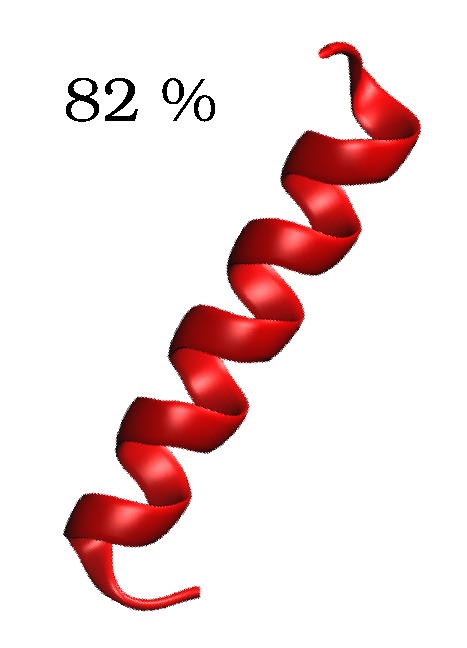
\includegraphics[height=4.5cm]{plots/helix6.pdf}
 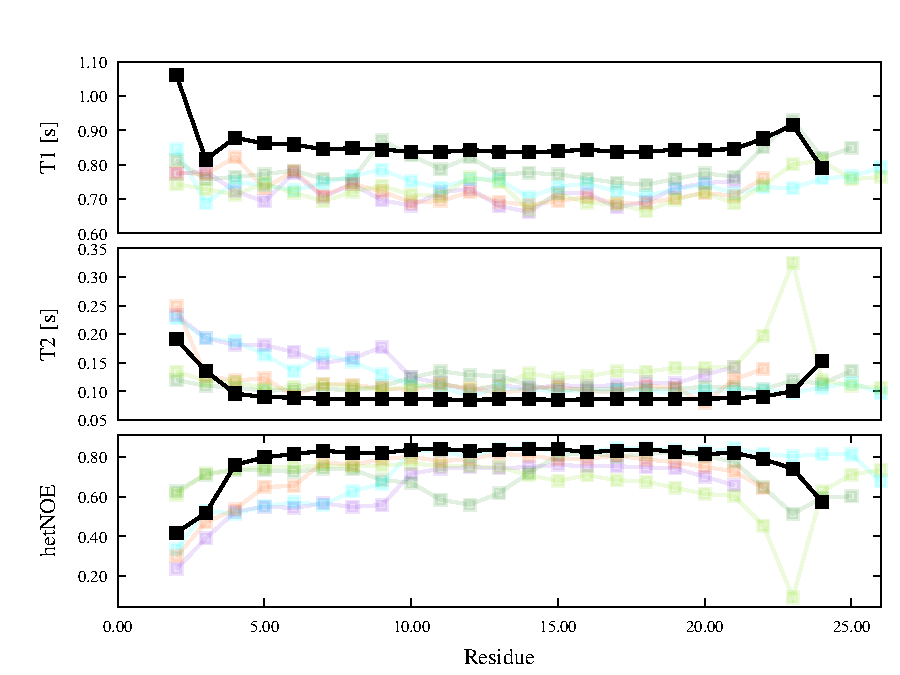
\includegraphics[height=5cm]{plots/simul_helix16.pdf}
 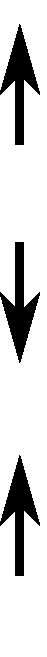
\includegraphics[height=4.5cm]{plots/arrows.pdf}
\end{center}

\end{frame}


\addtocounter{framenumber}{-1}
\begin{frame}
\LARGE{\centering
\textbf{Helicity correlates with relaxation times} \\}
\begin{center}
 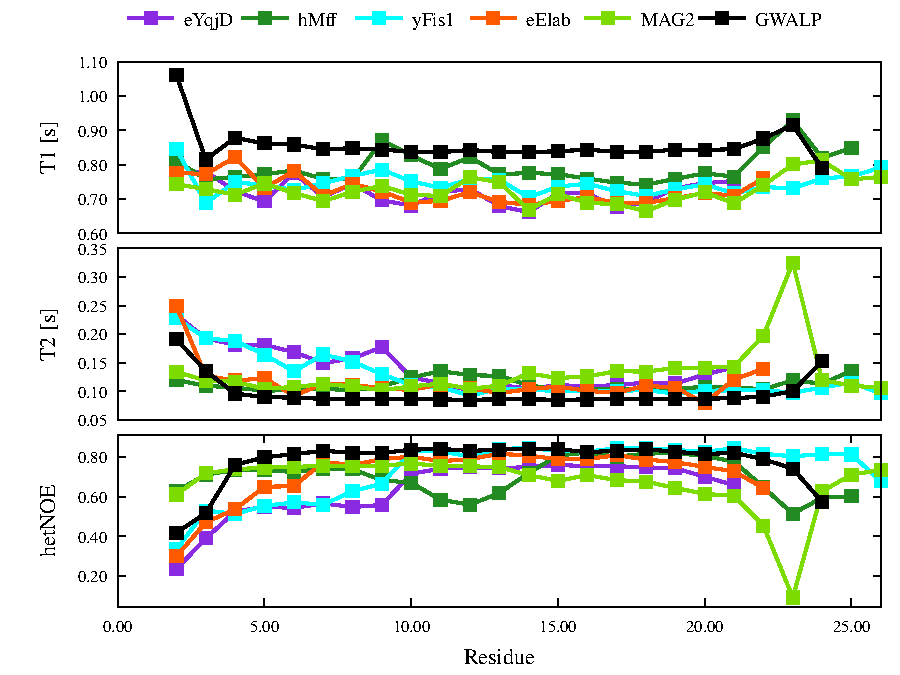
\includegraphics[height=6cm]{plots/simul_helix_all.pdf}
\end{center}

\end{frame}


\begin{frame}
\LARGE{\centering
\textbf{How to interpret relaxation times?} \\
\begin{center}
 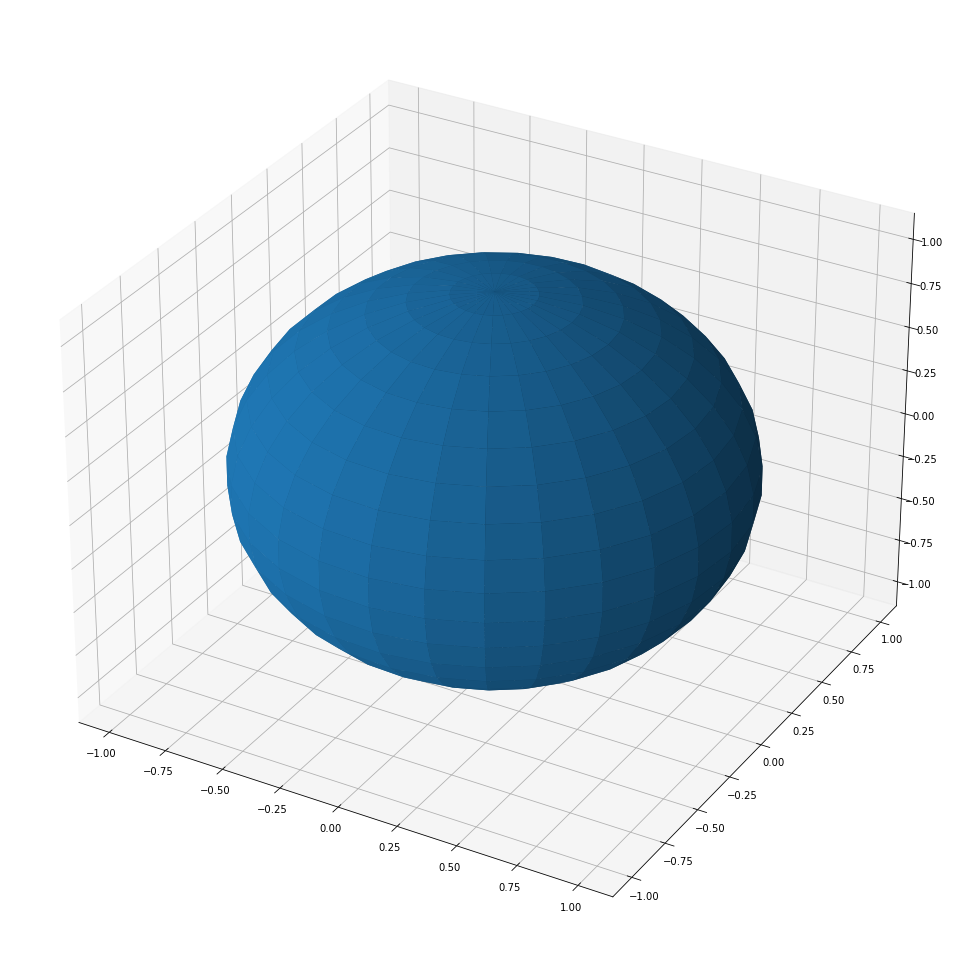
\includegraphics[height=5cm]{kolo.png}
\end{center}
T1, T2, hetNOE\\
}
{\tiny http://www.clker.com/clipart-animal-cell-3.html }
\end{frame}





%\begin{frame}
%\LARGE{\centering
%\textbf{A challenge to represent motionally averaged, sparse  pr ambiguous data with an ensemble of states}}
%\end{frame}


%\begin{frame}
%\LARGE{\centering
%\textbf{Structurally interpreting data obtained from most NMR dynamics experioments is complicated, however, because the signals are averaged over the ensamble populated in specific time windows}}
%\end{frame}


%\begin{frame}
%\LARGE{\centering
%\textbf{NOE distance restrains can be used for structure determination. But there is not sufficient info to determine relative populations of confoirmers in the ensamble}}
%\end{frame}







\begin{frame}
\LARGE{\centering
\textbf{Simulations fit experiments}}
\end{frame}




